\section{Waveform of PMT} % (fold)
PMT (Photomultiplier Tube) is a device which is highly sensitive to even single photon. Therefore, PMT is widely used in neutrino experiments based on liquid and dark matter experiment. In neutrino experiments, liquid scintillator emits light after excited by candidate particles and charged particles emit Cherenkov light in liquid. Timing resolution is crucial in neutrino event reconstruction. 

Timing resolution is determined by PMT and waveform analysis. Typical PMT response includes 3 individual processes: photo-electron conversion happened on photocathode. Electron collection by the first dynode. And amplification of electrons between dynodes. So 1 photon incoming has a certain probability to be observed via PMT voltage (See figure~\ref{fig:spe}). But if photons hit the PMT continually, the PE response will pile-up (see figure~\ref{fig:pile}) and the waveform analysis will be difficult. Pile-up will significantly worsen timing resolution. 

\begin{figure}[H]
\begin{minipage}{.5\textwidth}
\begin{figure}[H]
    \centering
    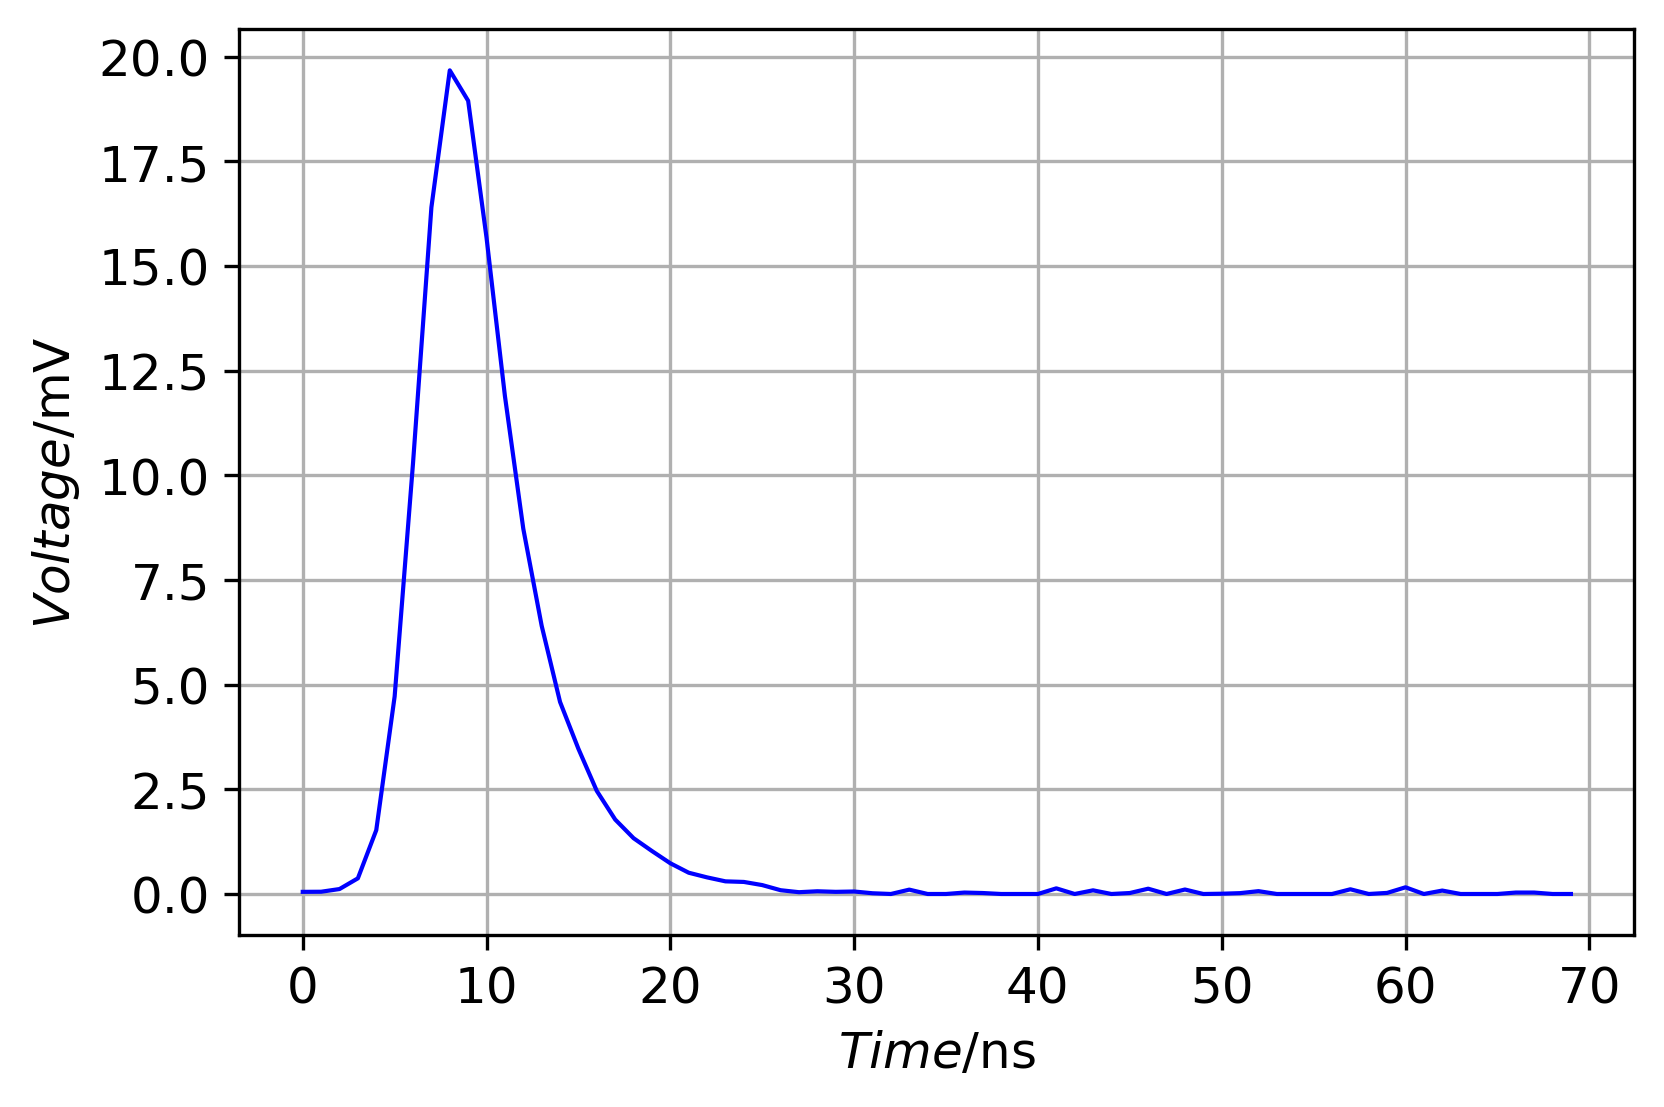
\includegraphics[width=1.0\linewidth]{figures/pmtspe.png}
    \caption{\label{fig:spe} PMT Single PE response}
\end{figure}
\end{minipage}
\begin{minipage}{.5\textwidth}
\begin{figure}[H]
    \centering
    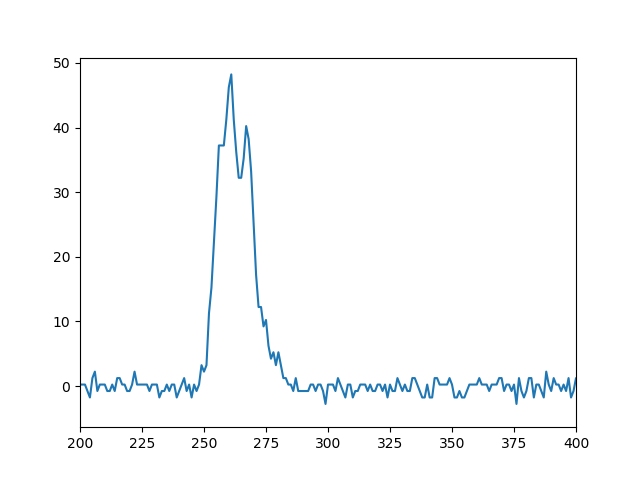
\includegraphics[width=1.0\linewidth]{figures/wave.png}
    \caption{\label{fig:pile} Pile-up in waveform}
\end{figure}
\end{minipage}
\end{figure}

Naively, when handling PMT waveform we record the first hittime according to threshold and the integration of waveform. One waveform is converted to a pair of numbers. More detailed information of the waveform (see figure~\ref{fig:tradi}) was lost. The new goal in this work is to extract information of all hits in 1 DAQ window including HitTime (the time when electron hit the first dynode) \& Charge or \#PE (number of photo-electrons in specific time, see figure~\ref{fig:new}). The time we defined here is discrete value in 1 window of data-taking (from 0 to 1029ns in 1ton prototype data-taking system). 

\begin{figure}[H]
\begin{minipage}{.5\textwidth}
\begin{figure}[H]
    \centering
    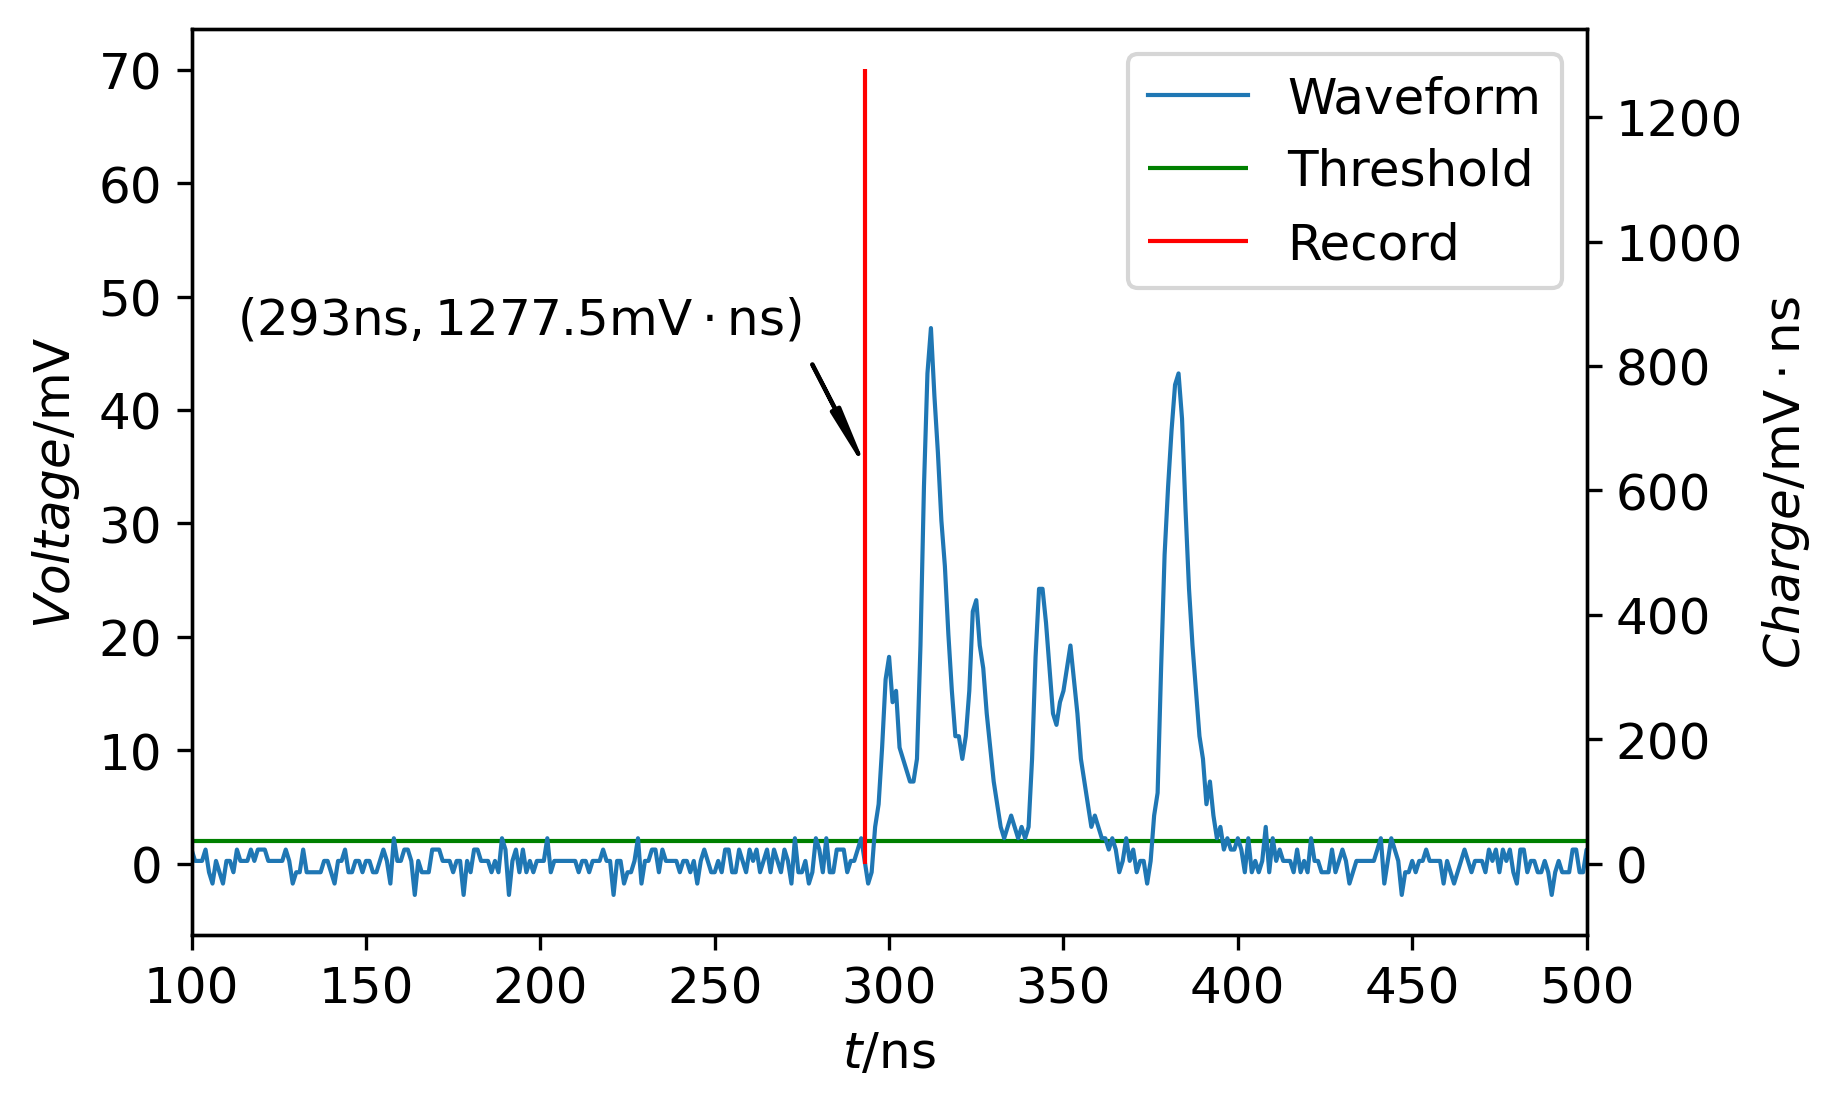
\includegraphics[width=1.0\linewidth]{figures/previous.png}
    \caption{\label{fig:tradi} Traditional Recorded Waveform}
\end{figure}
\end{minipage}
\begin{minipage}{.5\textwidth}
\begin{figure}[H]
    \centering
    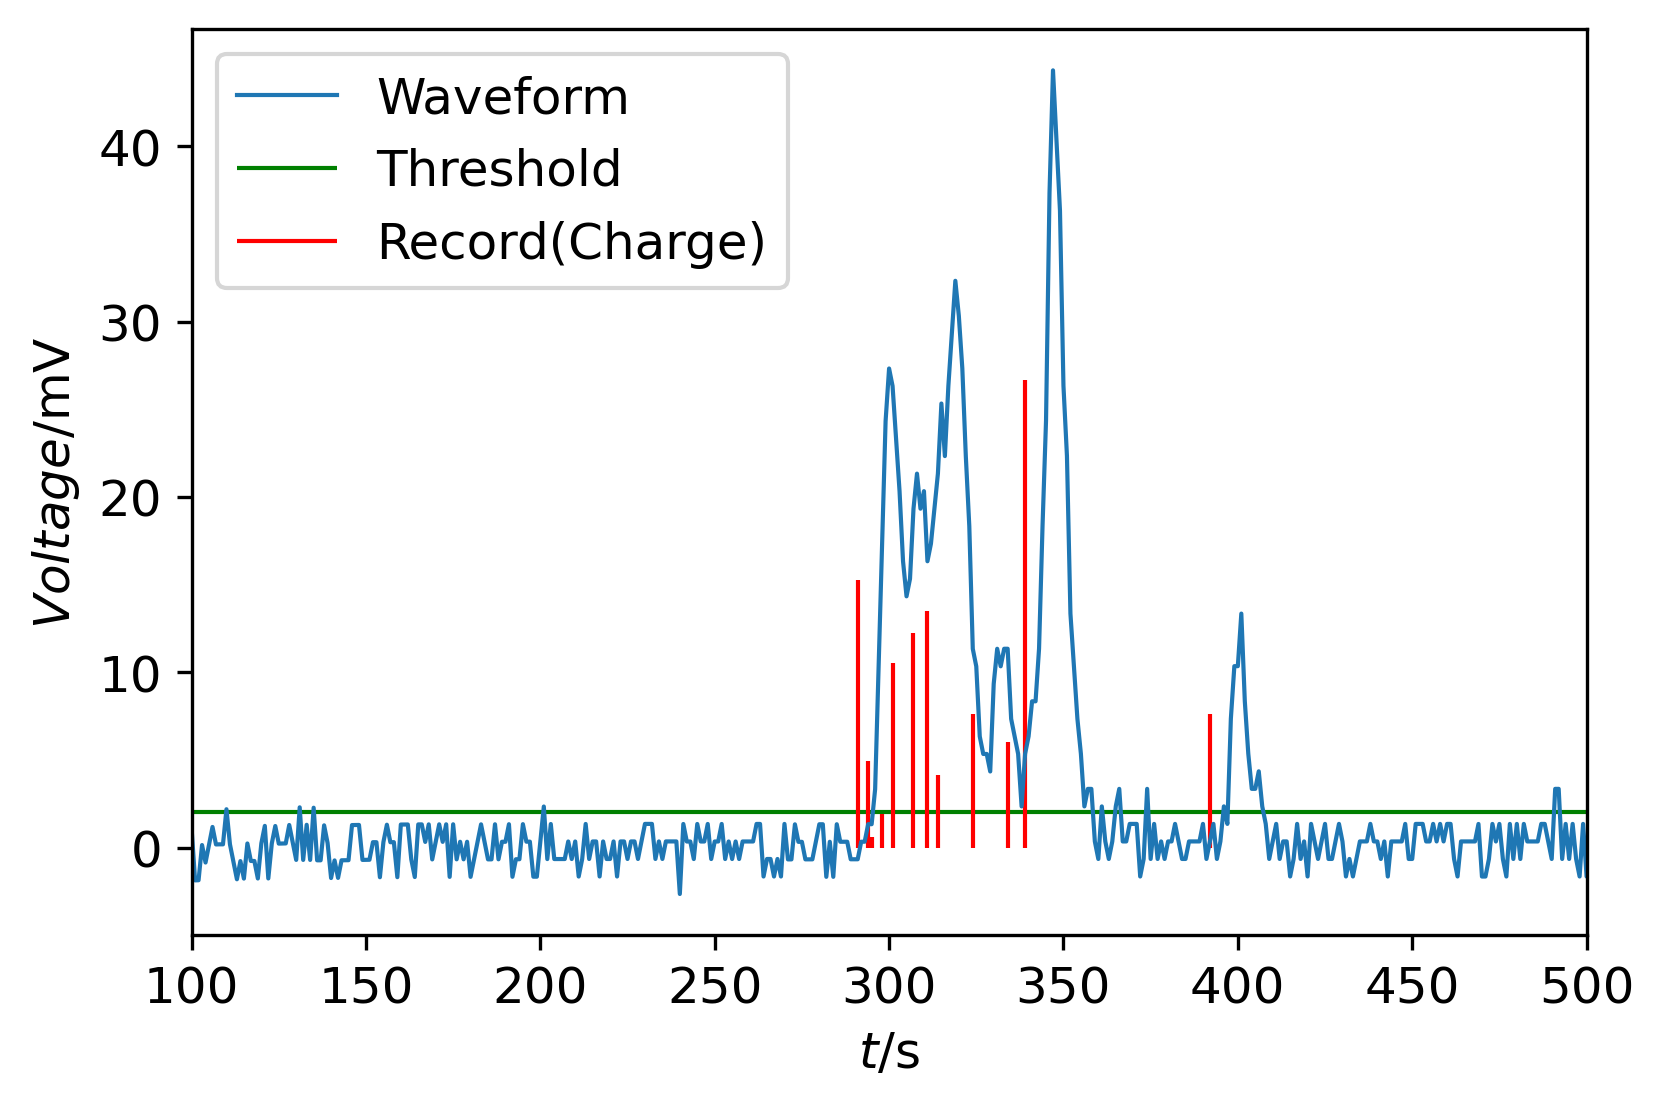
\includegraphics[width=1.0\linewidth]{figures/goal.png}
    \caption{\label{fig:new} New Goal Recorded Waveform}
\end{figure}
\end{minipage}
\end{figure}

Charge is the integration of waveform component which induced by single photo-electron. Single PE induced charge can be a wide distribution, rather than a single value. Reconstructing \#PE is more difficult than reconstructing Charge. 

\begin{figure}[H]
    \centering
    \includegraphics[width=0.6\linewidth]{figures/chargehist.png}
    \caption{\label{fig:charge} Distribution of Charge}
\end{figure}

% section Waveform of PMT (end)